% !TEX root = paper.tex
\appendix
\section{Model comparisons of the Individual flow harmonics $v_n$}
\label{sec:vn}
As discussed in Sec.~\ref{sec:method}, NSC$(m,n)$ is expected to be insensitive to the magnitudes of $v_{m}$ and $v_{n}$ but SC$(m,n)$ has contributions from both the correlations between the two different flow harmonics and the individual harmonics $v_{n}$. Therefore it is important to check how well the theoretical models used in Sec.~\ref{sec:theory} describe the measured $v_n$ data shown in Sec.~\ref{sec:results}. The comparisons are made only up to $v_4$ because model calculations are not available for $v_5$ at this moment. %to date
\begin{figure*}[h]
            \begin{center}
                       \resizebox{0.34\textwidth}{!}{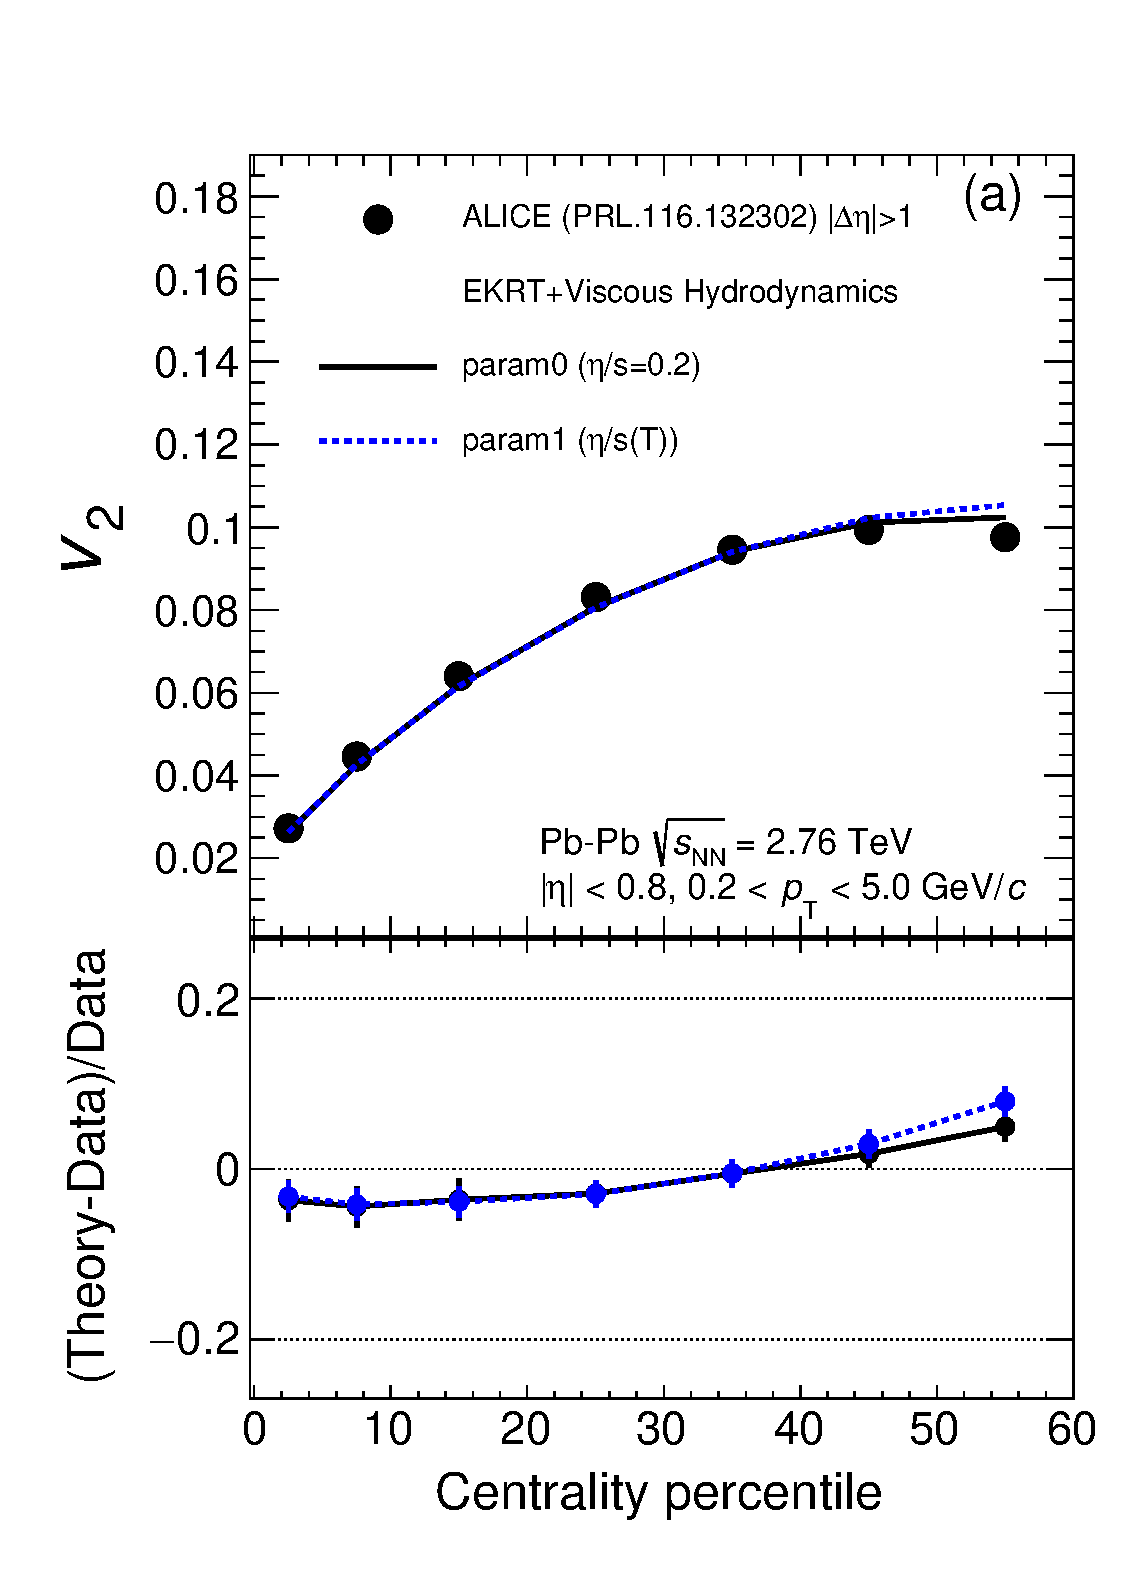
\includegraphics{figs/FigA1_v2_comp_EKRT.eps}}\hspace{-0.27cm}
                       \resizebox{0.34\textwidth}{!}{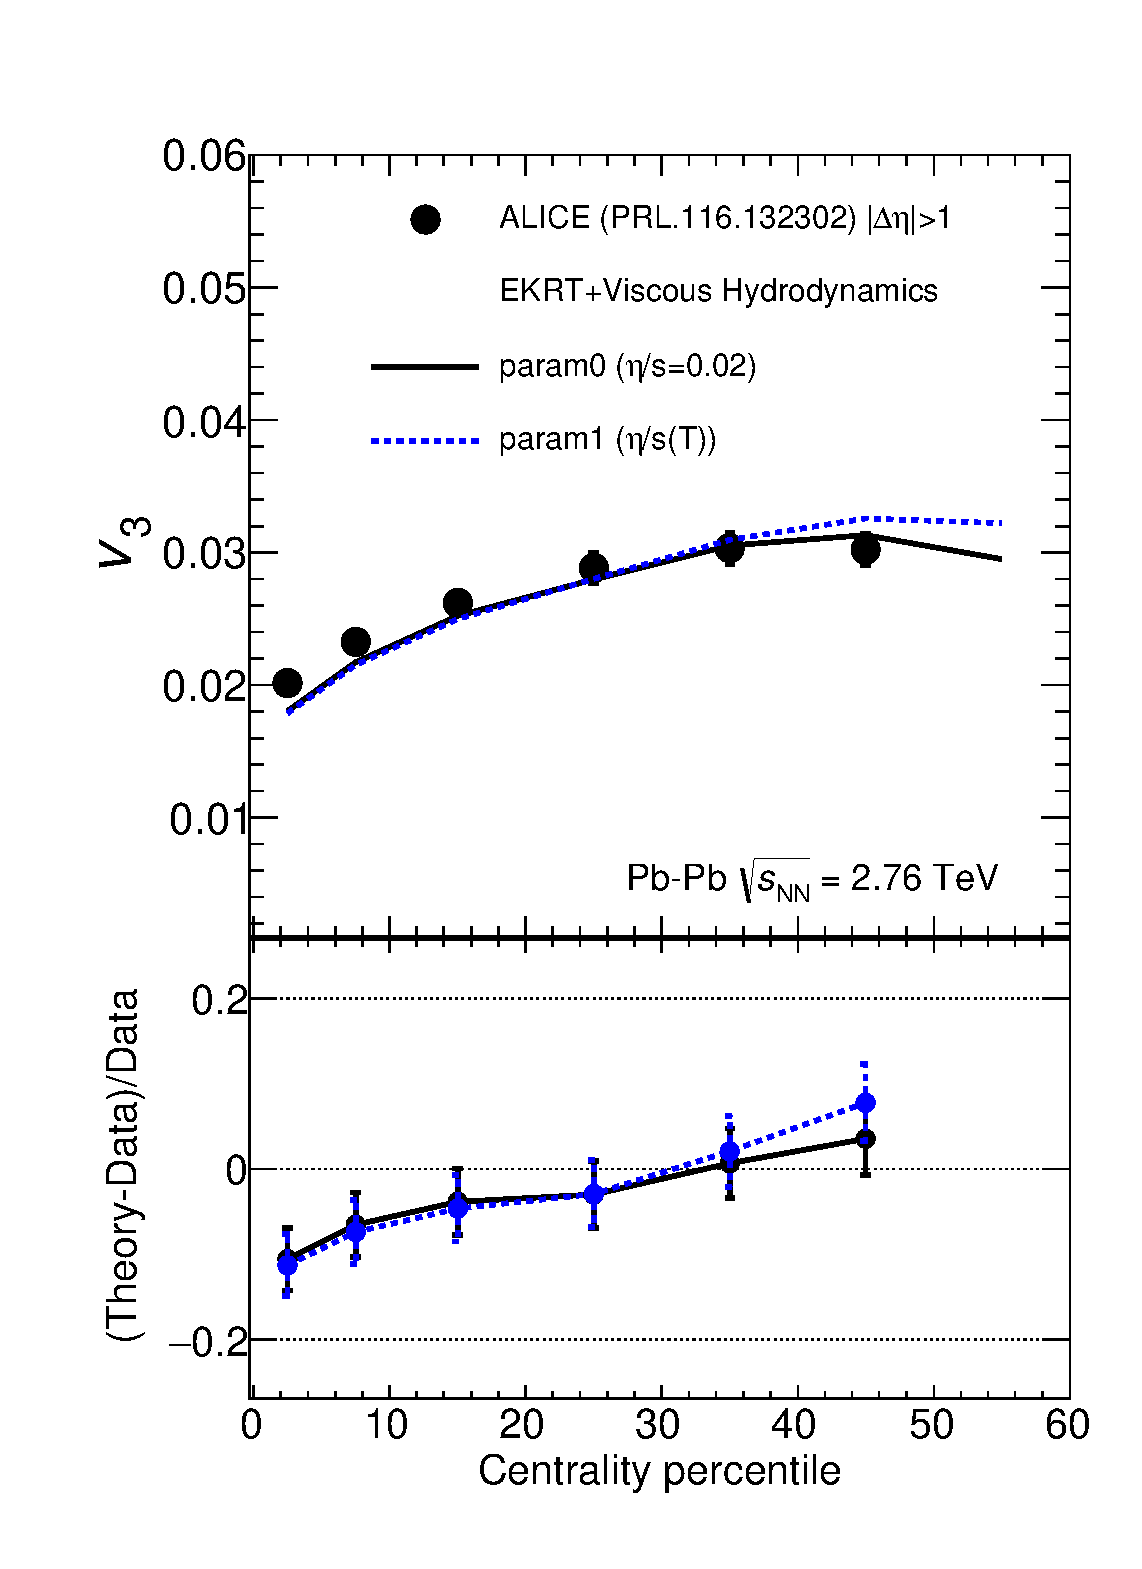
\includegraphics{figs/FigA1_v3_comp_EKRT.eps}}\hspace{-0.27cm}
                       \resizebox{0.34\textwidth}{!}{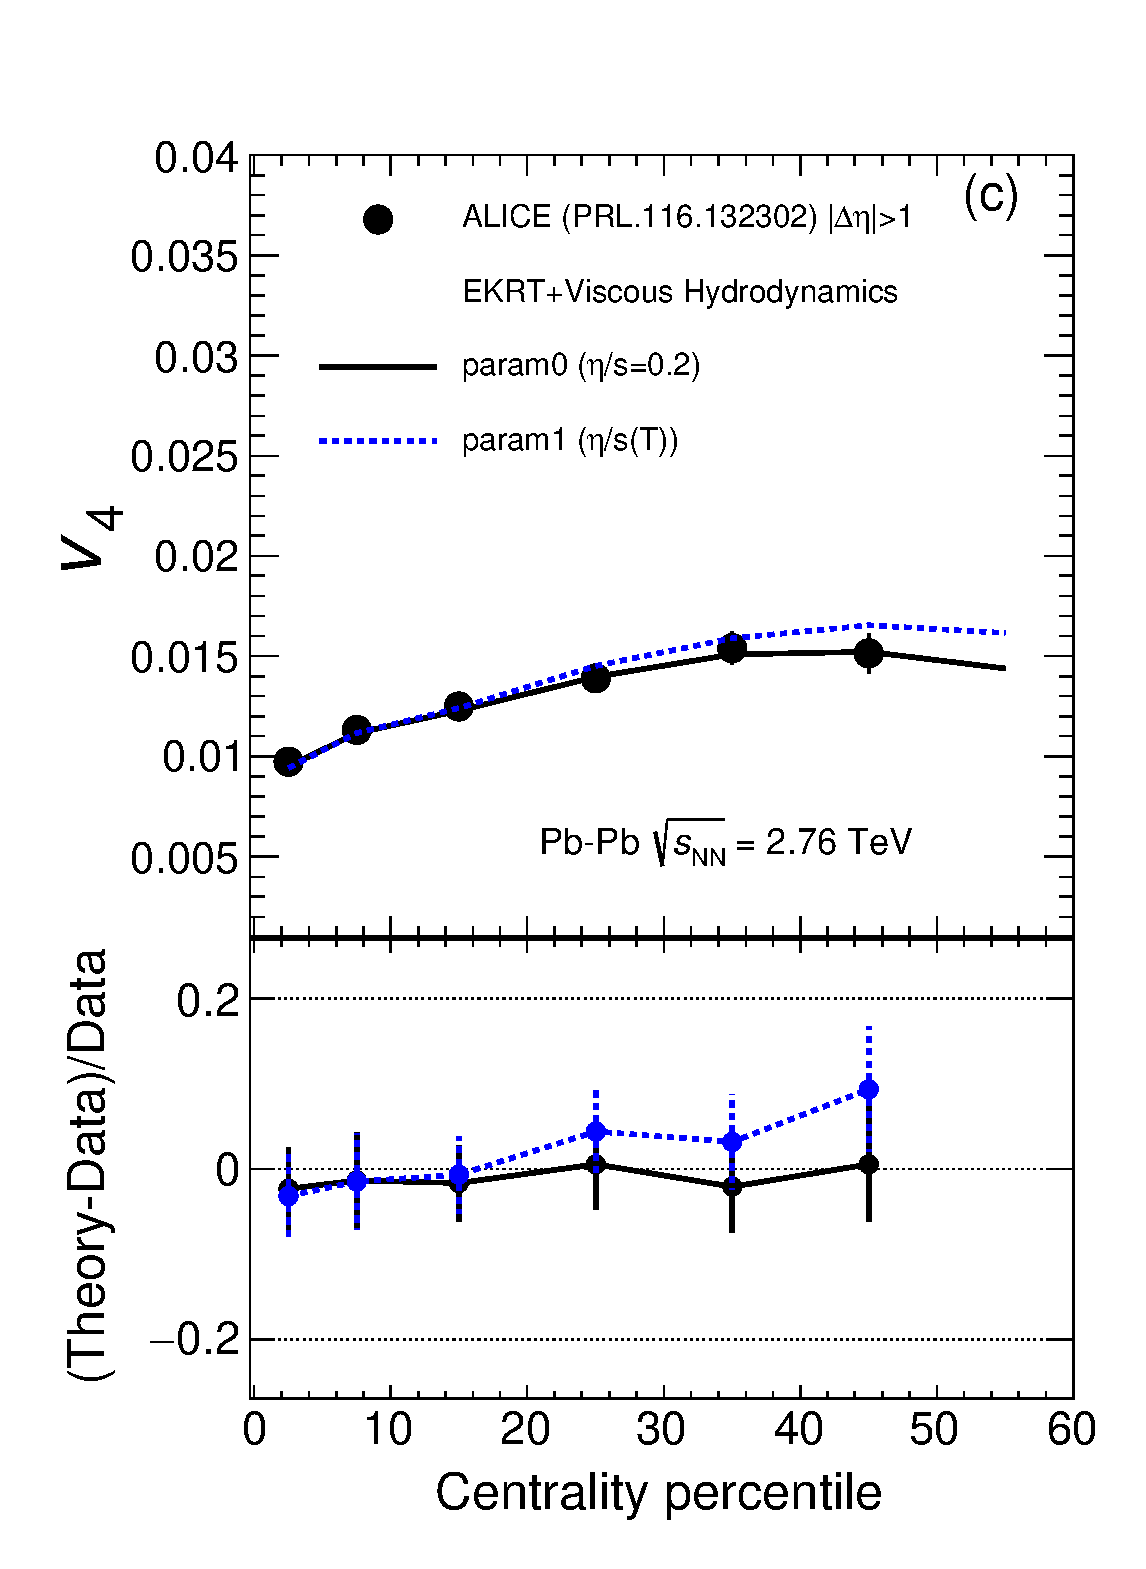
\includegraphics{figs/FigA1_v4_comp_EKRT.eps}}
        \caption{The individual flow harmonics $v_n$ (n=2, 3 and 4) in $\PbPb$ collisions at $\snn=2.76$~TeV~\cite{Adam:2016izf} are compared to the event-by-event EKRT+viscous hydrodynamic calculations~\cite{Niemi:2015qia}. The lines are hydrodynamic predictions with two different $\eta/s(T)$ parameterizations, labeled in the same way as in ~\cite{Niemi:2015qia}.}
        \label{fig:Figure_A1}
              \end{center}
\end{figure*}

The measured $v_n$ (n=2, 3 and 4) in $\PbPb$ collisions at $\snn=2.76$~TeV are compared to the event-by-event EKRT+viscous hydrodynamic calculations~\cite{Niemi:2015qia} in Fig.~\ref{fig:Figure_A1}. In these calculations the initial conditions and $\eta/s$ parameterizations are chosen to reproduce the LHC $v_n$ data.
The calculations captures the centrality dependence of $v_n$ in the central and midcentral collisions within 5\% for $v_2$ and 10\% for $v_3$ and $v_4$.

\begin{figure*}[h]
            \begin{center}
                       \resizebox{0.34\textwidth}{!}{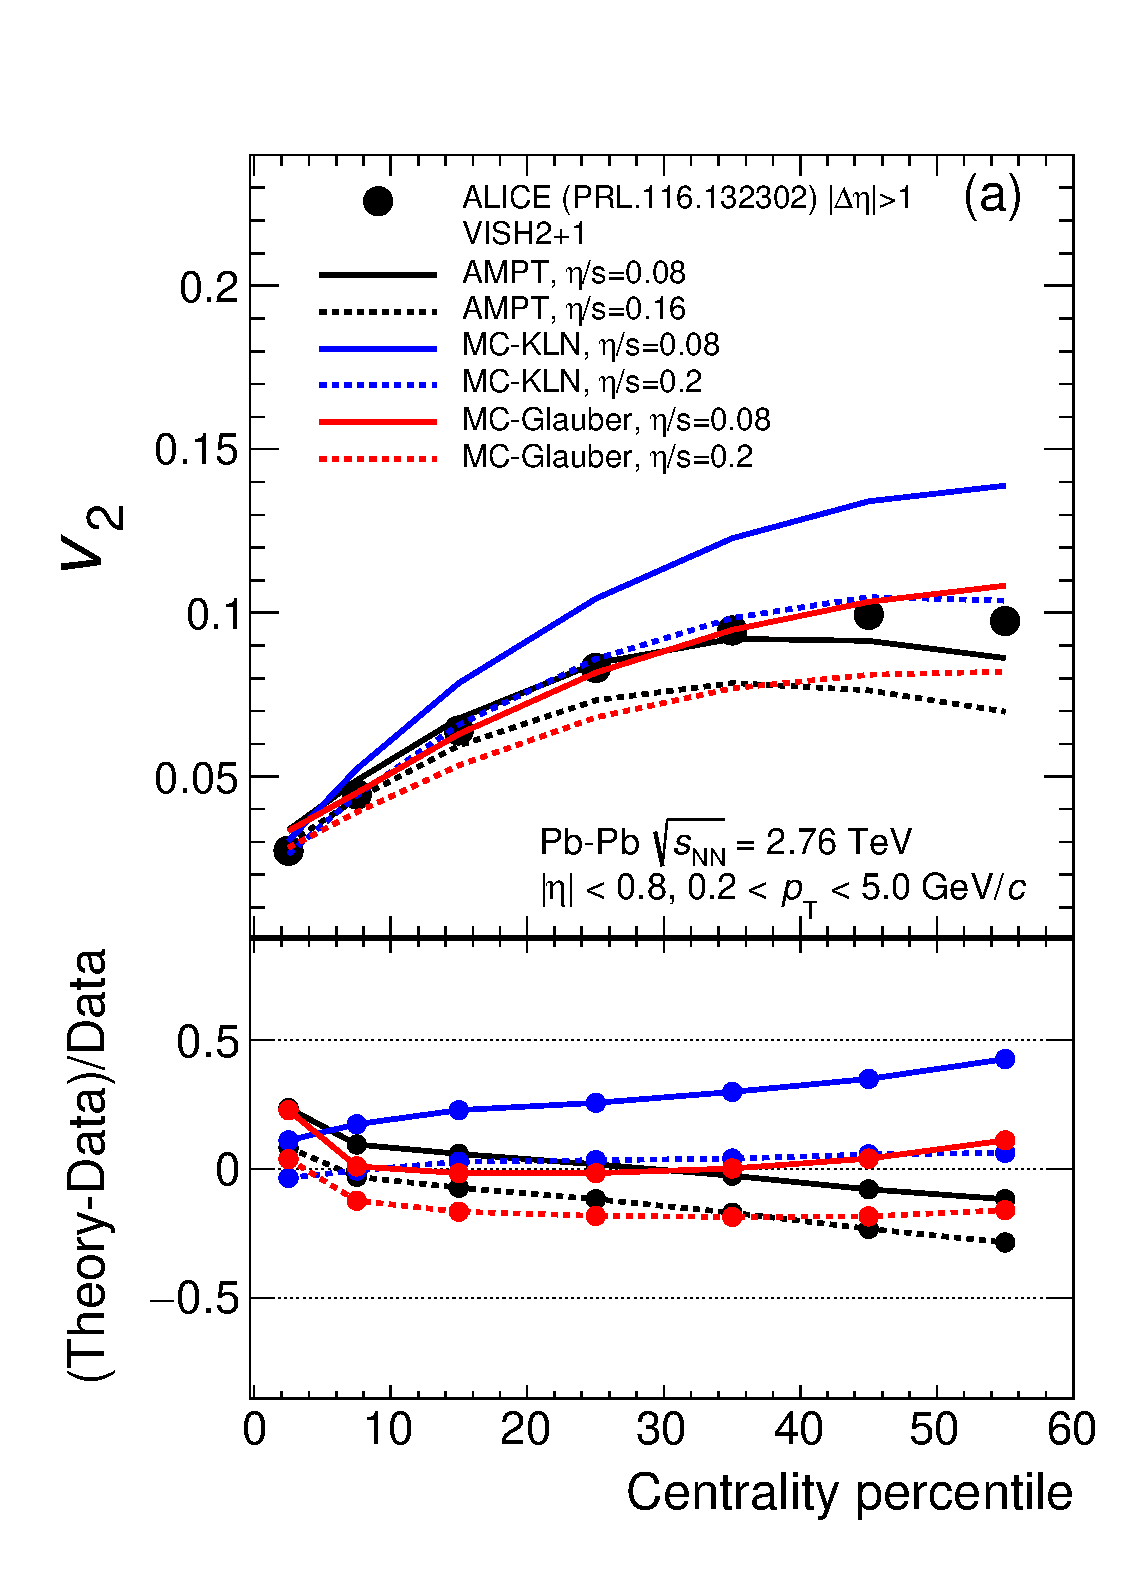
\includegraphics{figs/FigA2_v2_comp_VISH.eps}}\hspace{-0.27cm}
                       \resizebox{0.34\textwidth}{!}{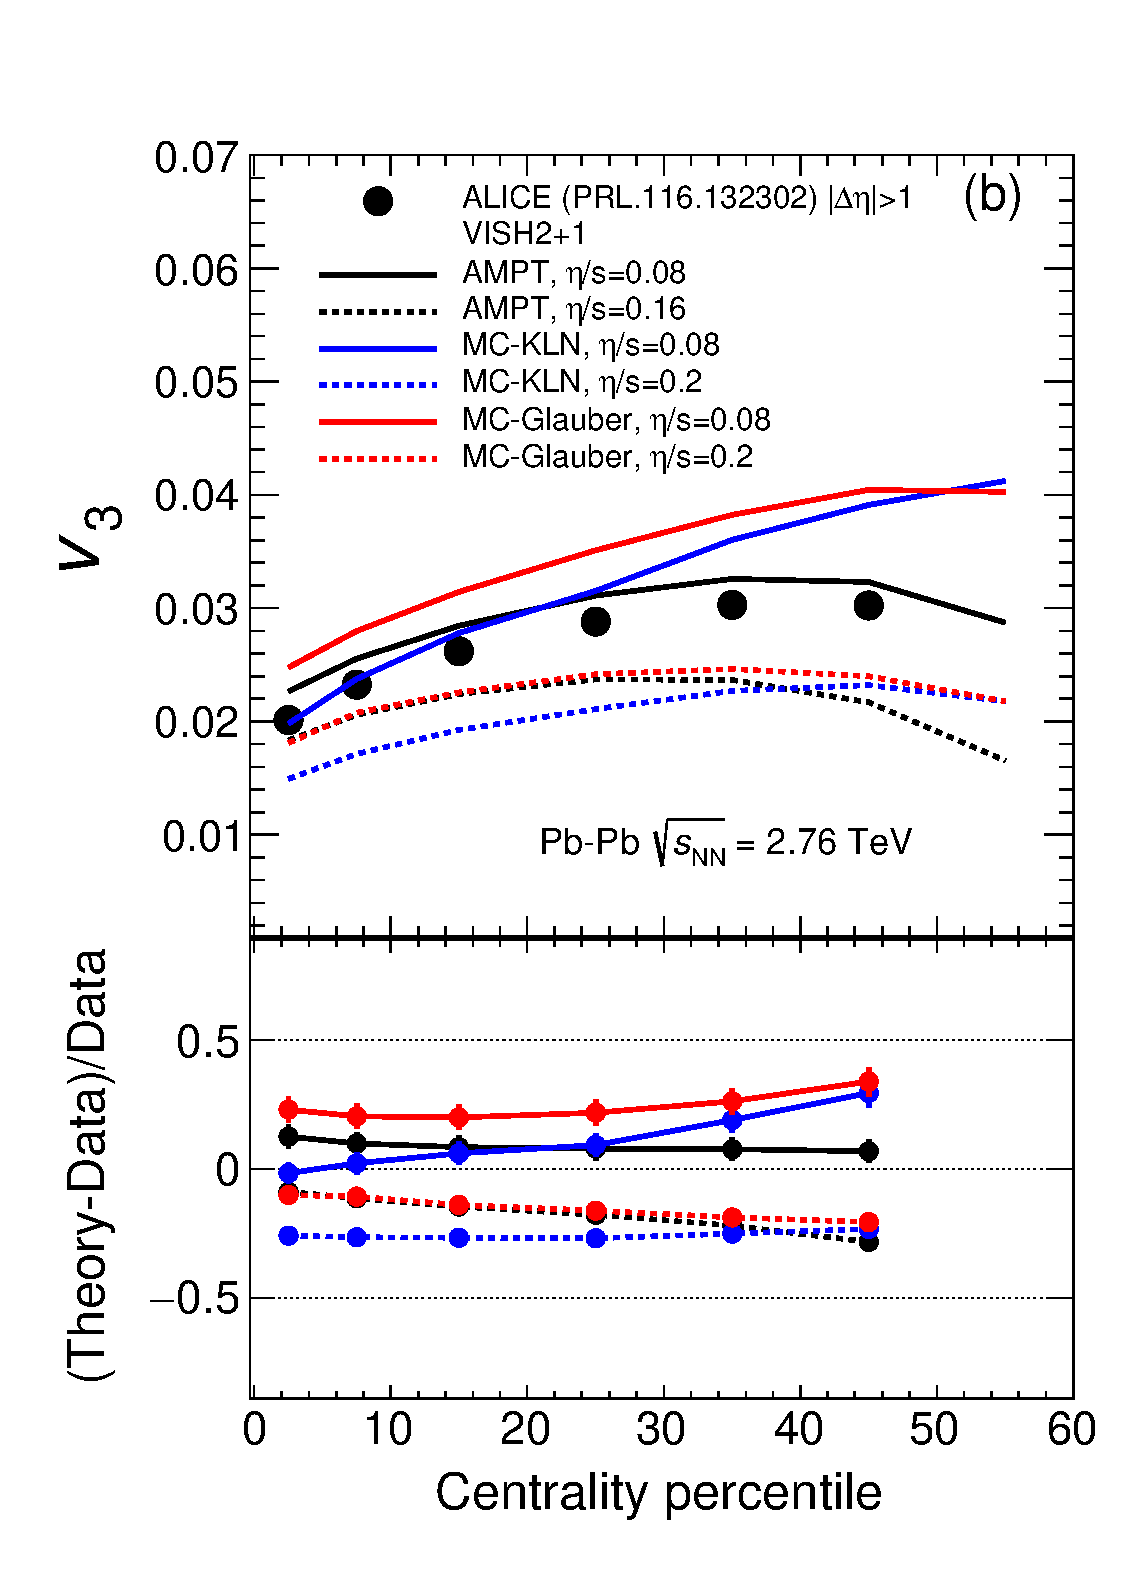
\includegraphics{figs/FigA2_v3_comp_VISH.eps}}\hspace{-0.27cm}
                       \resizebox{0.34\textwidth}{!}{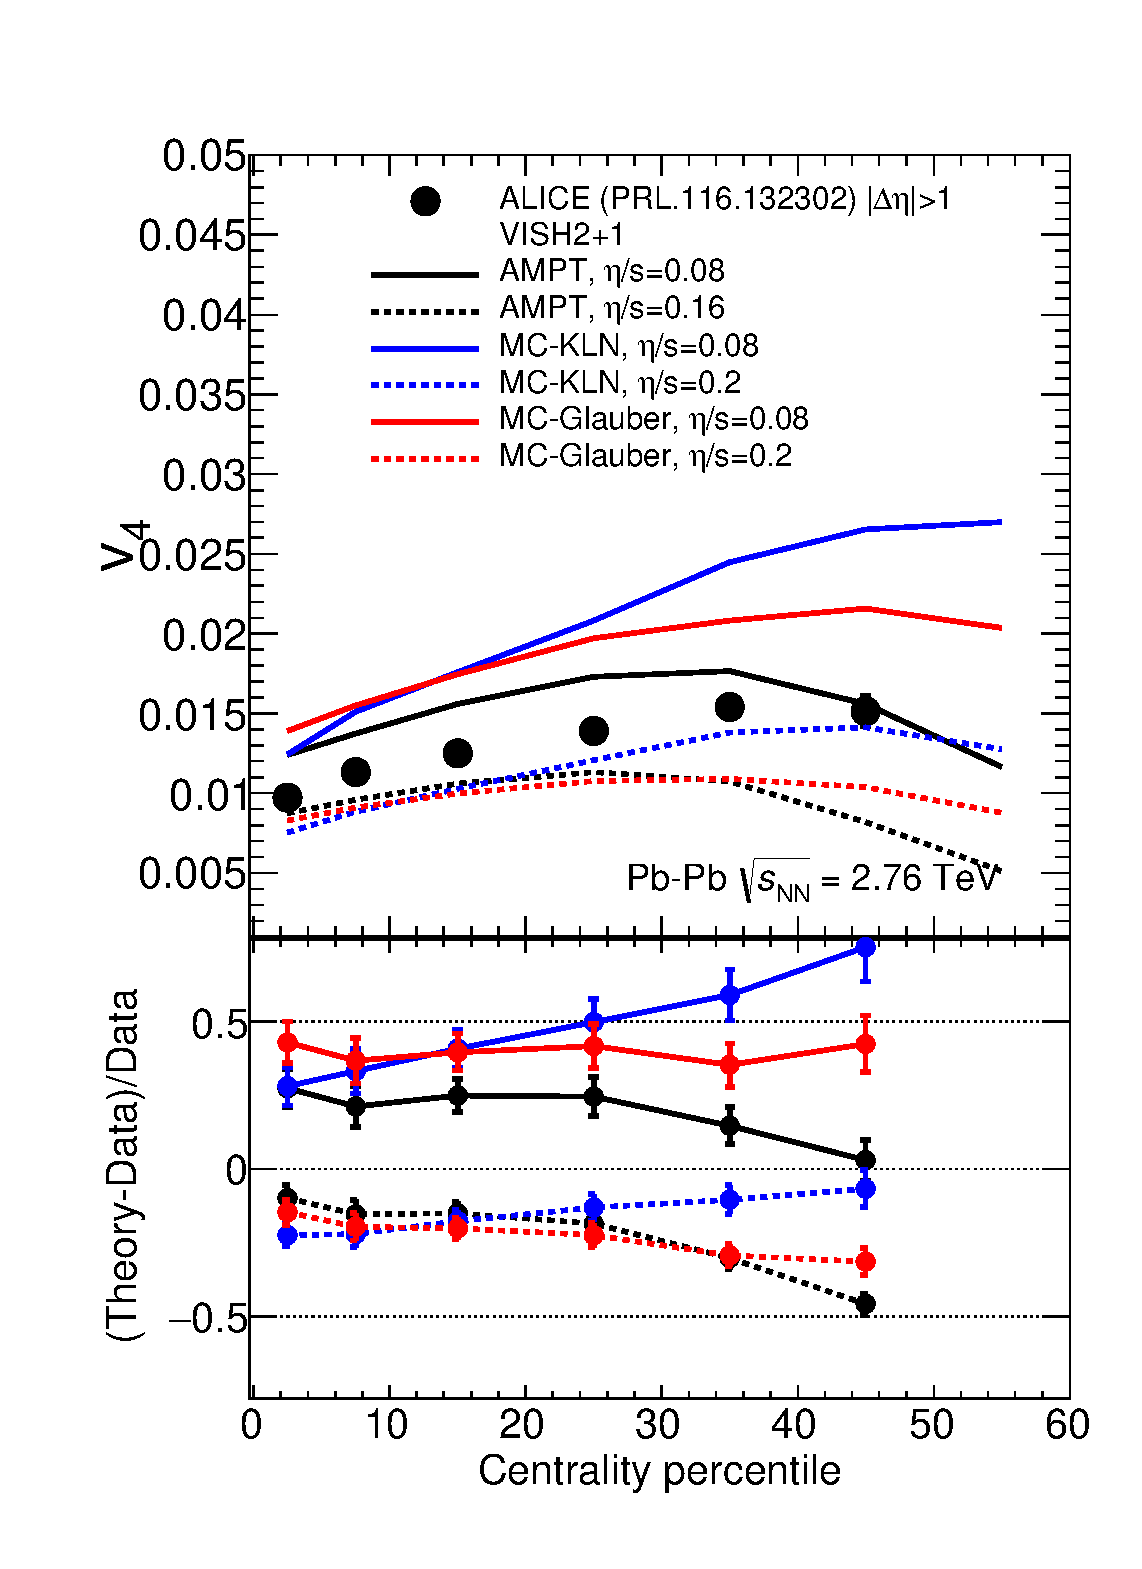
\includegraphics{figs/FigA2_v4_comp_VISH.eps}}
        \caption{The individual flow harmonics $v_n$ (n=2, 3 and 4) in $\PbPb$ collisions at $\snn=2.76$~TeV~\cite{Adam:2016izf} are compared to various VISH2+1 calculations~\cite{Zhu:2016puf}. Three initial conditions from AMPT, MC-KLN and MC-Glauber are drawn as different colors. The $\eta/s$ parameters are shown as different line styles, the small shear viscosity ($\eta/s=0.08$) are shown as solid lines, and large shear viscosities ($\eta/s=0.2$ for MC-KLN and MC-Glauber, 0.16 for AMPT) are drawn as dashed lines.}
        \label{fig:Figure_A2}
              \end{center}
\end{figure*}

The VISH2+1 calculations with various initial conditions and $\eta/s$ parameters are compared to the $v_n$ data in Fig.~\ref{fig:Figure_A2}.
Neither MC-Glauber nor MC-KLN initial conditions can simultaneously describe $v_2$, $v_3$ and $v_4$. In particular, for MC-Glauber initial conditions, VISH2+1 with $\eta/s$ = 0.08 could nicely describe $v_2$ from central to midcentral collisions, but overestimates $v_3$ and $v_4$ for the same centrality ranges. For MC-KLN initial conditions, VISH2+1 with $\eta/s$ = 0.20 reproduces $v_2$ but underestimates $v_3$ and $v_4$ for the presented centrality regions. The calculations with AMPT initial conditions improves the simultaneous descriptions of $v_n$ (n = 2, 3 and 4). Overall difference to the data is quite large if all the model settings are considered, about 30\% for $v_n$ (n = 2 and 3),  50\% for $v_4$. The calculations with AMPT initial conditions reproduce the observed centrality dependence with the accuracy of 10-20\%.

\begin{figure*}[h]
            \begin{center}
                       \resizebox{0.34\textwidth}{!}{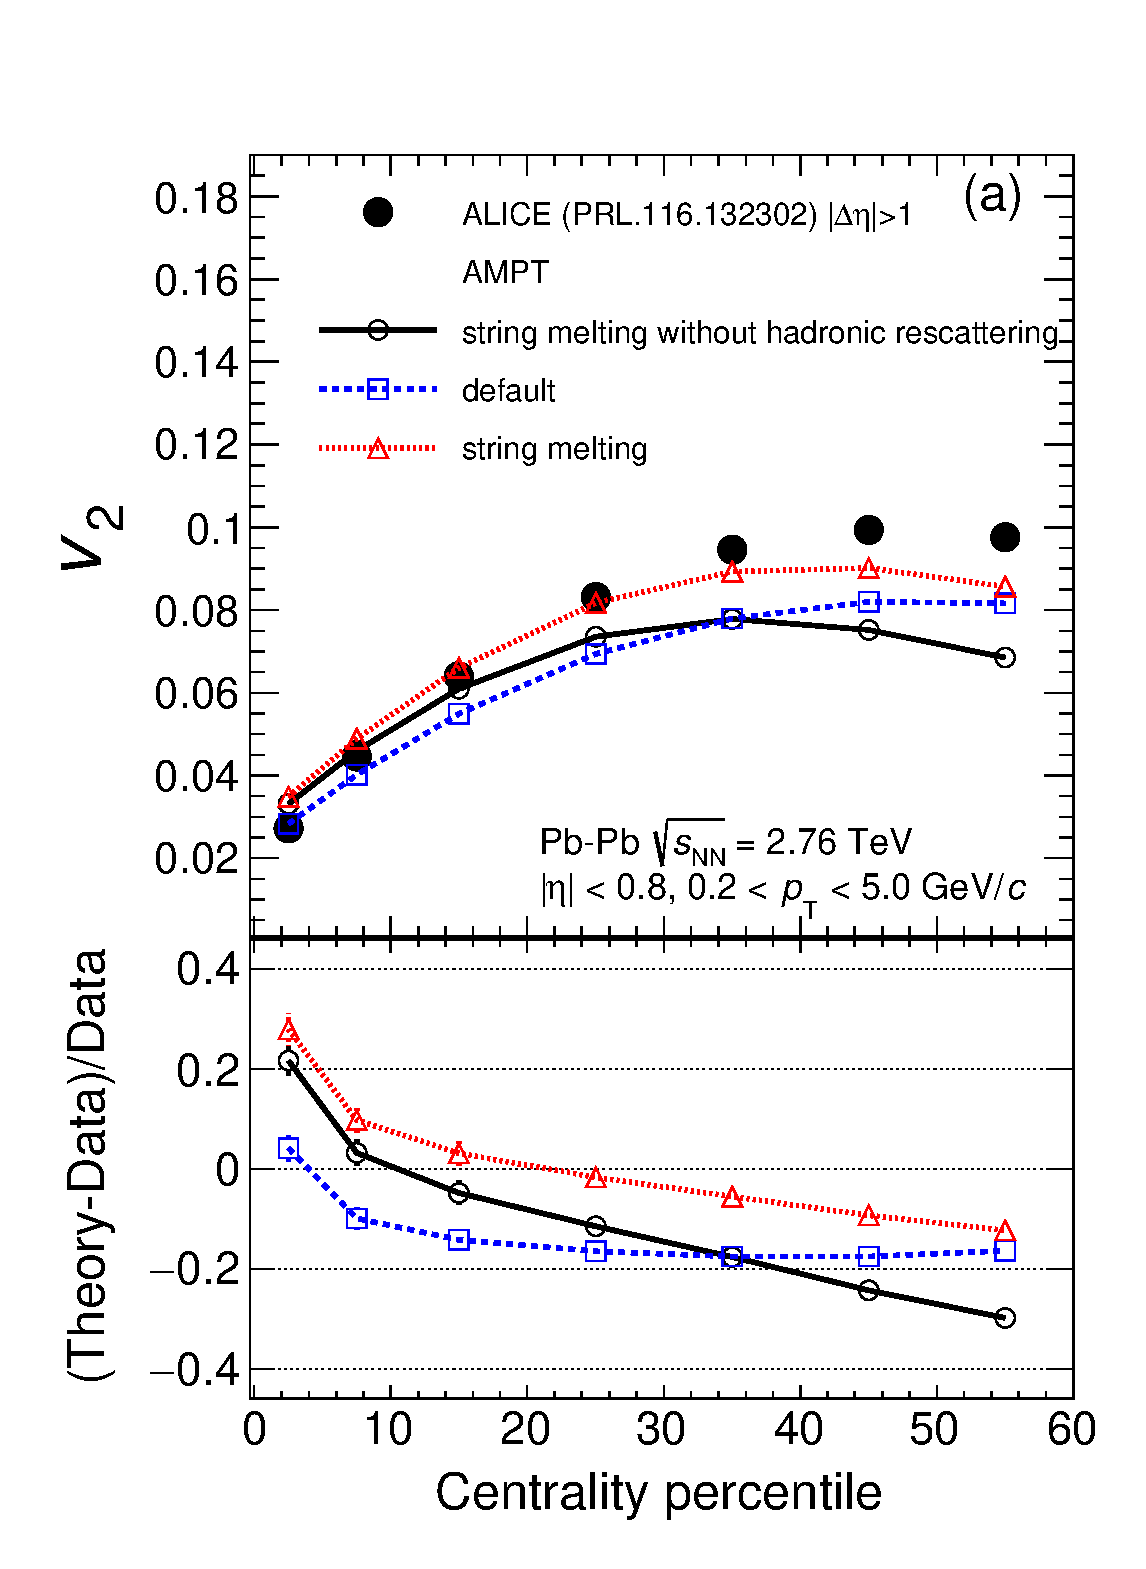
\includegraphics{figs/FigA3_v2_comp_AMPT.eps}}\hspace{-0.27cm}
                       \resizebox{0.34\textwidth}{!}{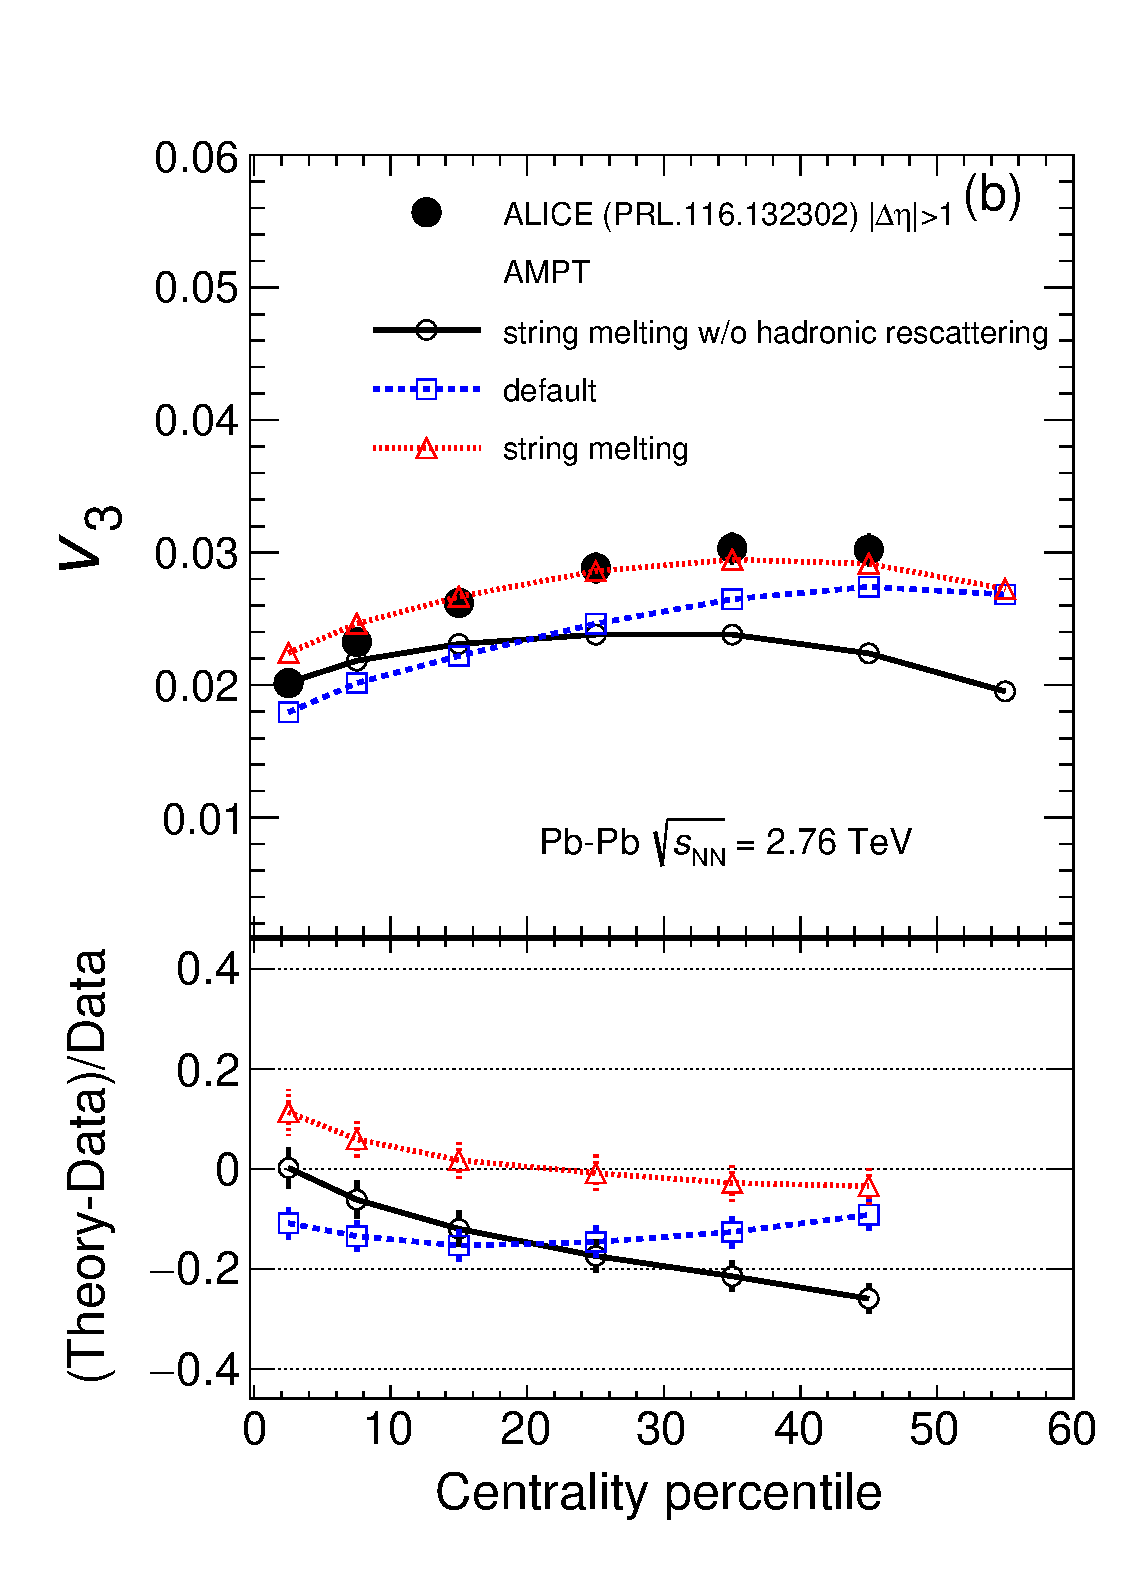
\includegraphics{figs/FigA3_v3_comp_AMPT.eps}}\hspace{-0.27cm}
                       \resizebox{0.34\textwidth}{!}{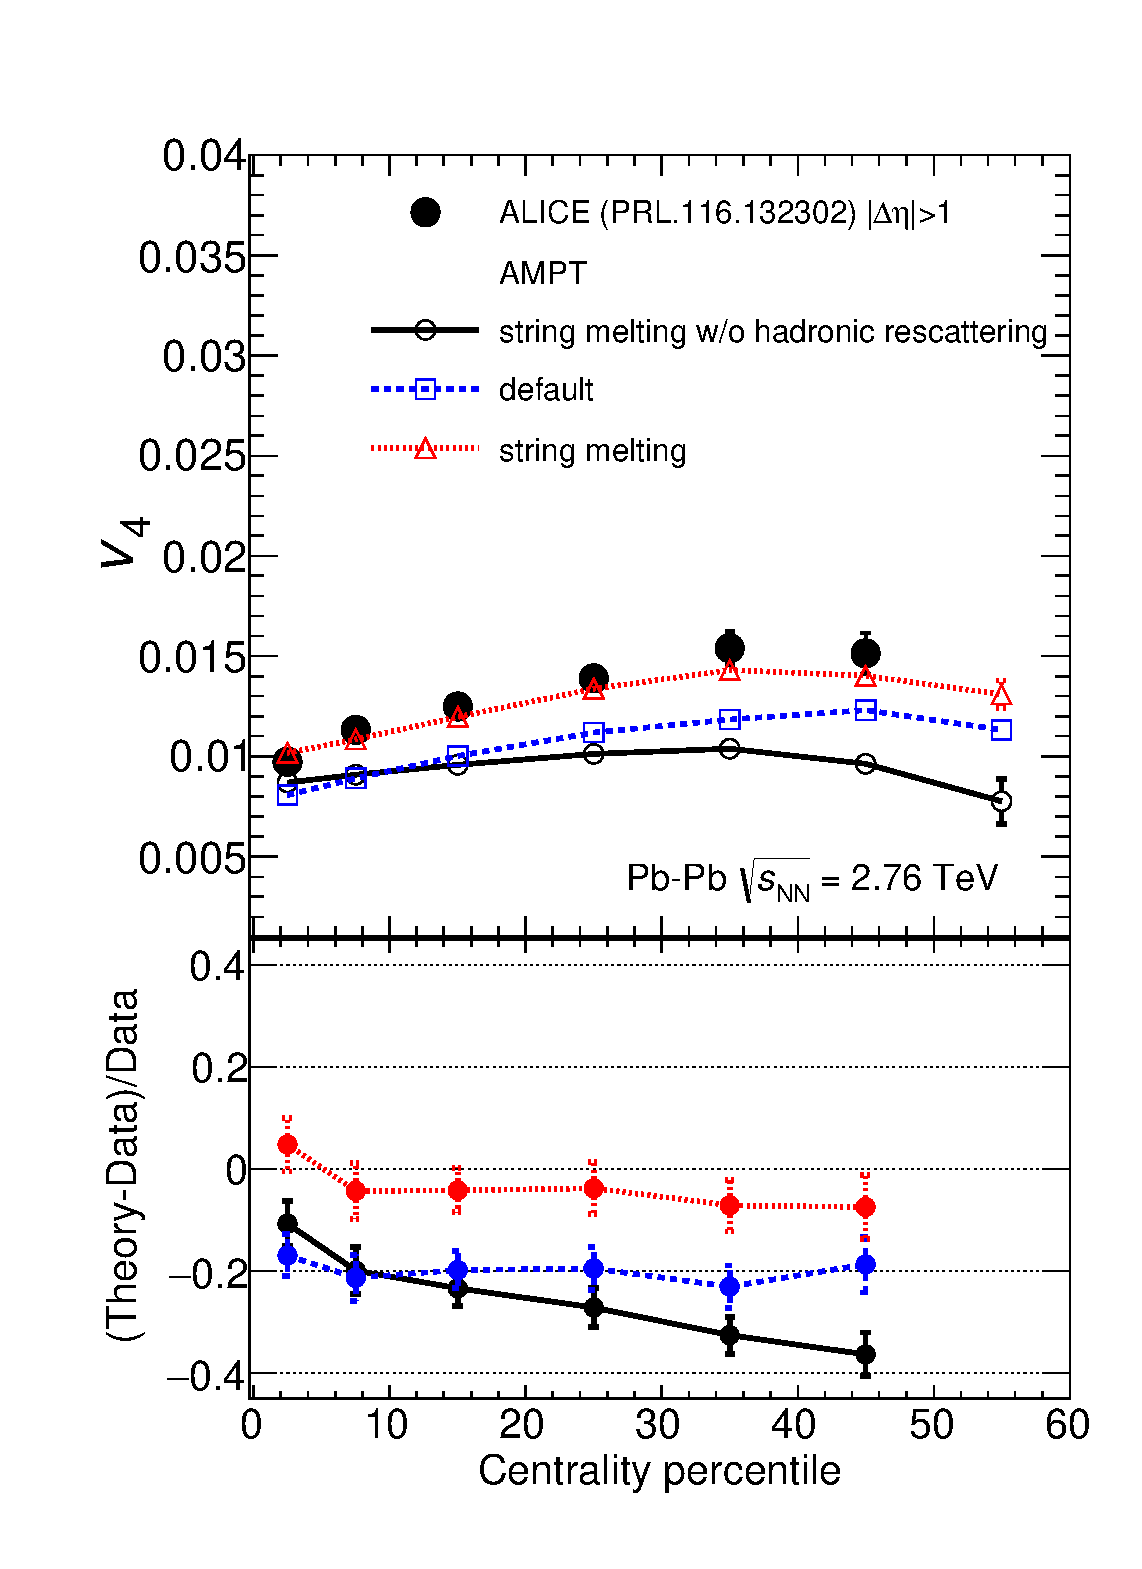
\includegraphics{figs/FigA3_v4_comp_AMPT.eps}}
        \caption{The individual flow harmonics $v_n$ (n=2, 3 and 4) in $\PbPb$ collisions at $\snn=2.76$~TeV~\cite{Adam:2016izf} are compared to various AMPT models.}
        \label{fig:Figure_A3}
              \end{center}
\end{figure*}

The AMPT calculations with various configurations are compared to the $v_n$ data in Fig.~\ref{fig:Figure_10}.
The string melting version of AMPT~\cite{Lin:2001zk,Lin:2004en} reasonably reproduces $v_n$ as shown in Fig.~\ref{fig:Figure_10} within 20\% for $v_2$ and 10\% for $v_3$ and $v_4$. The version based on the string melting configuration without the hadronic rescattering phase underestimates the data quite a bit compared to the calculations with the string melting version of AMPT, which demonstrates that a large fraction of the flow is developed during the late hadronic rescattering stage in the string melting version of AMPT.
The default version of AMPT underestimates $v_n$ (n = 2, 3 and 4) by $\approx$ 20\%. It should be noted that the default AMPT model can describe the normalized symmetric cumulants (NSC($m$,$n$)) quantitively for most centralities while the string melting AMPT model fails to describe them.

\begin{figure*}[h]
            \begin{center}
                       \resizebox{0.34\textwidth}{!}{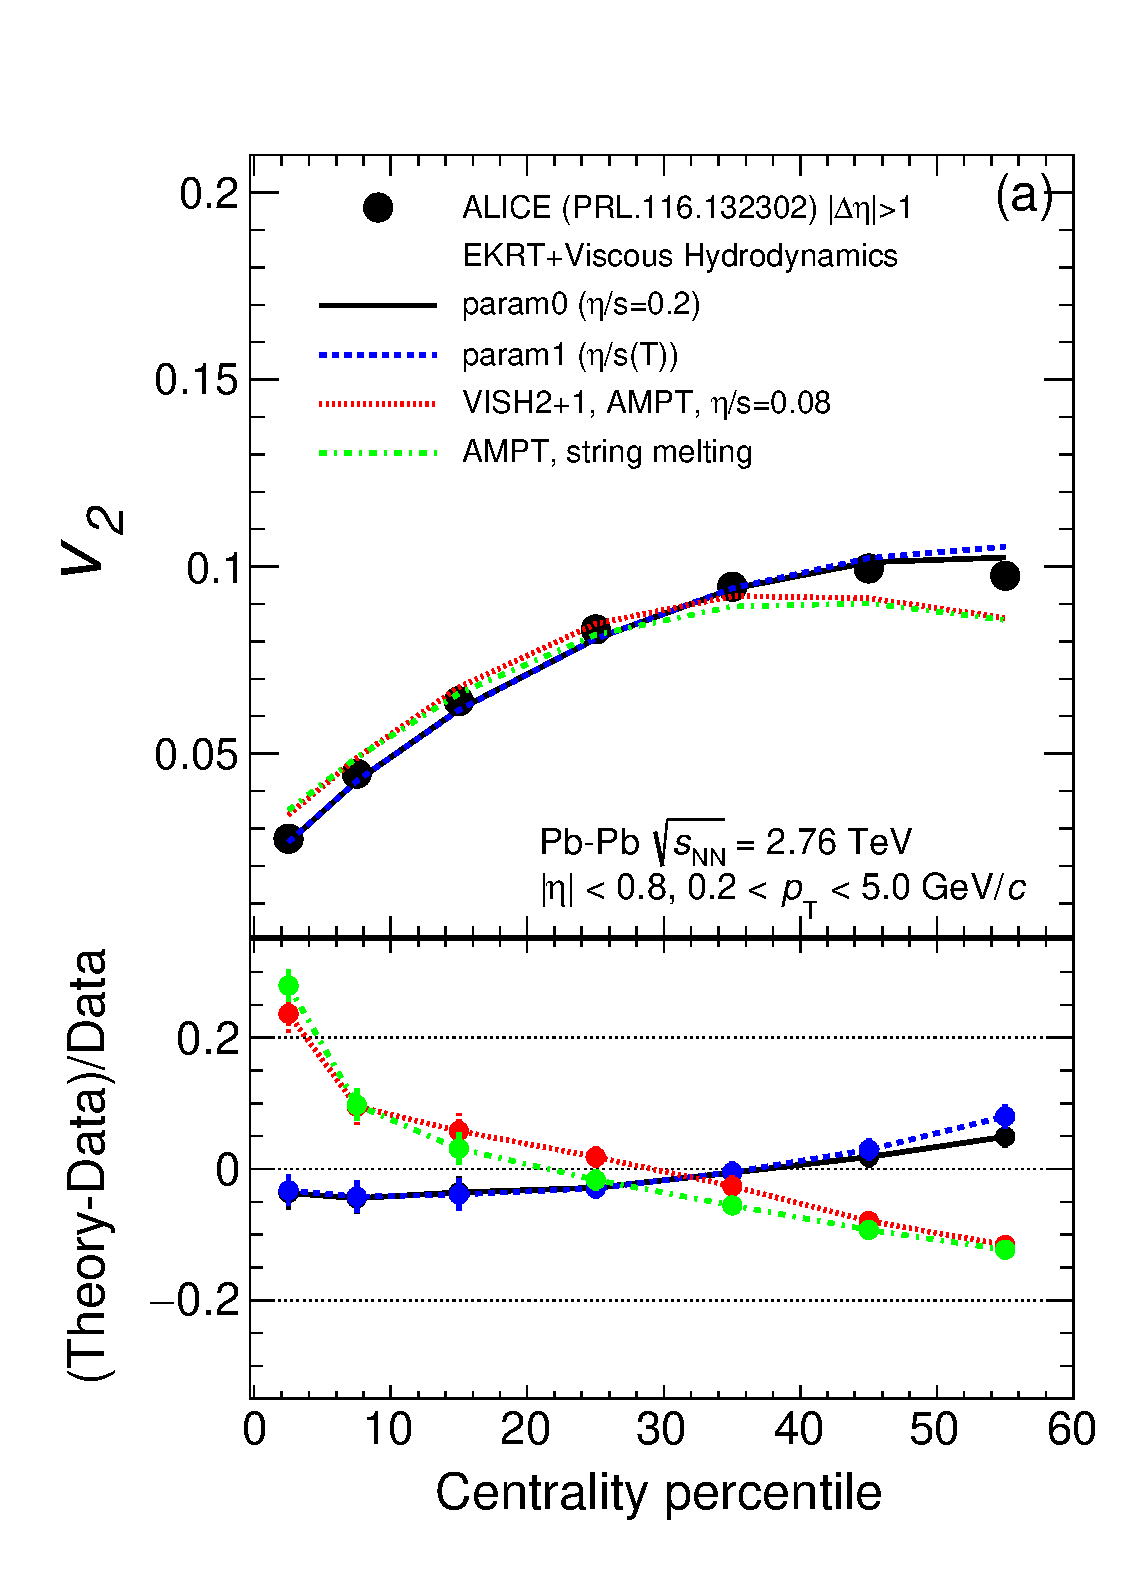
\includegraphics{figs/FigA4_v2_modelcomparisonBest.eps}}\hspace{-0.27cm}
                       \resizebox{0.34\textwidth}{!}{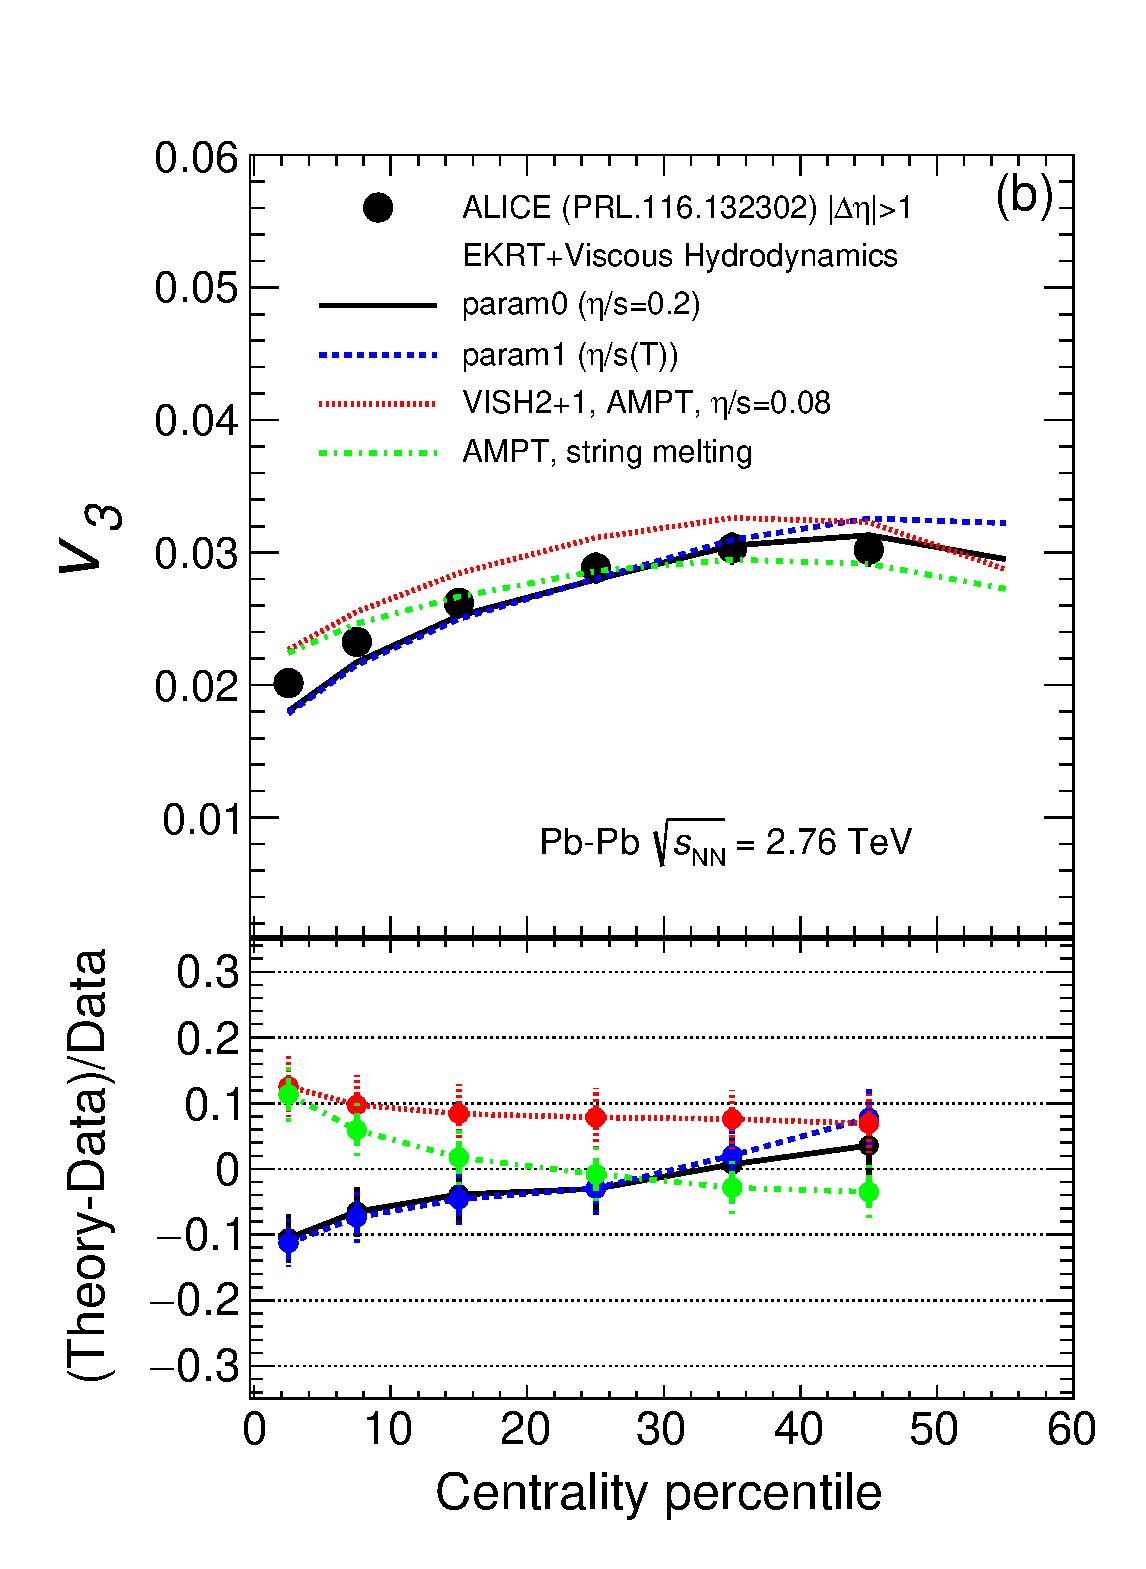
\includegraphics{figs/FigA4_v3_modelcomparisonBest.eps}}\hspace{-0.27cm}
                       \resizebox{0.34\textwidth}{!}{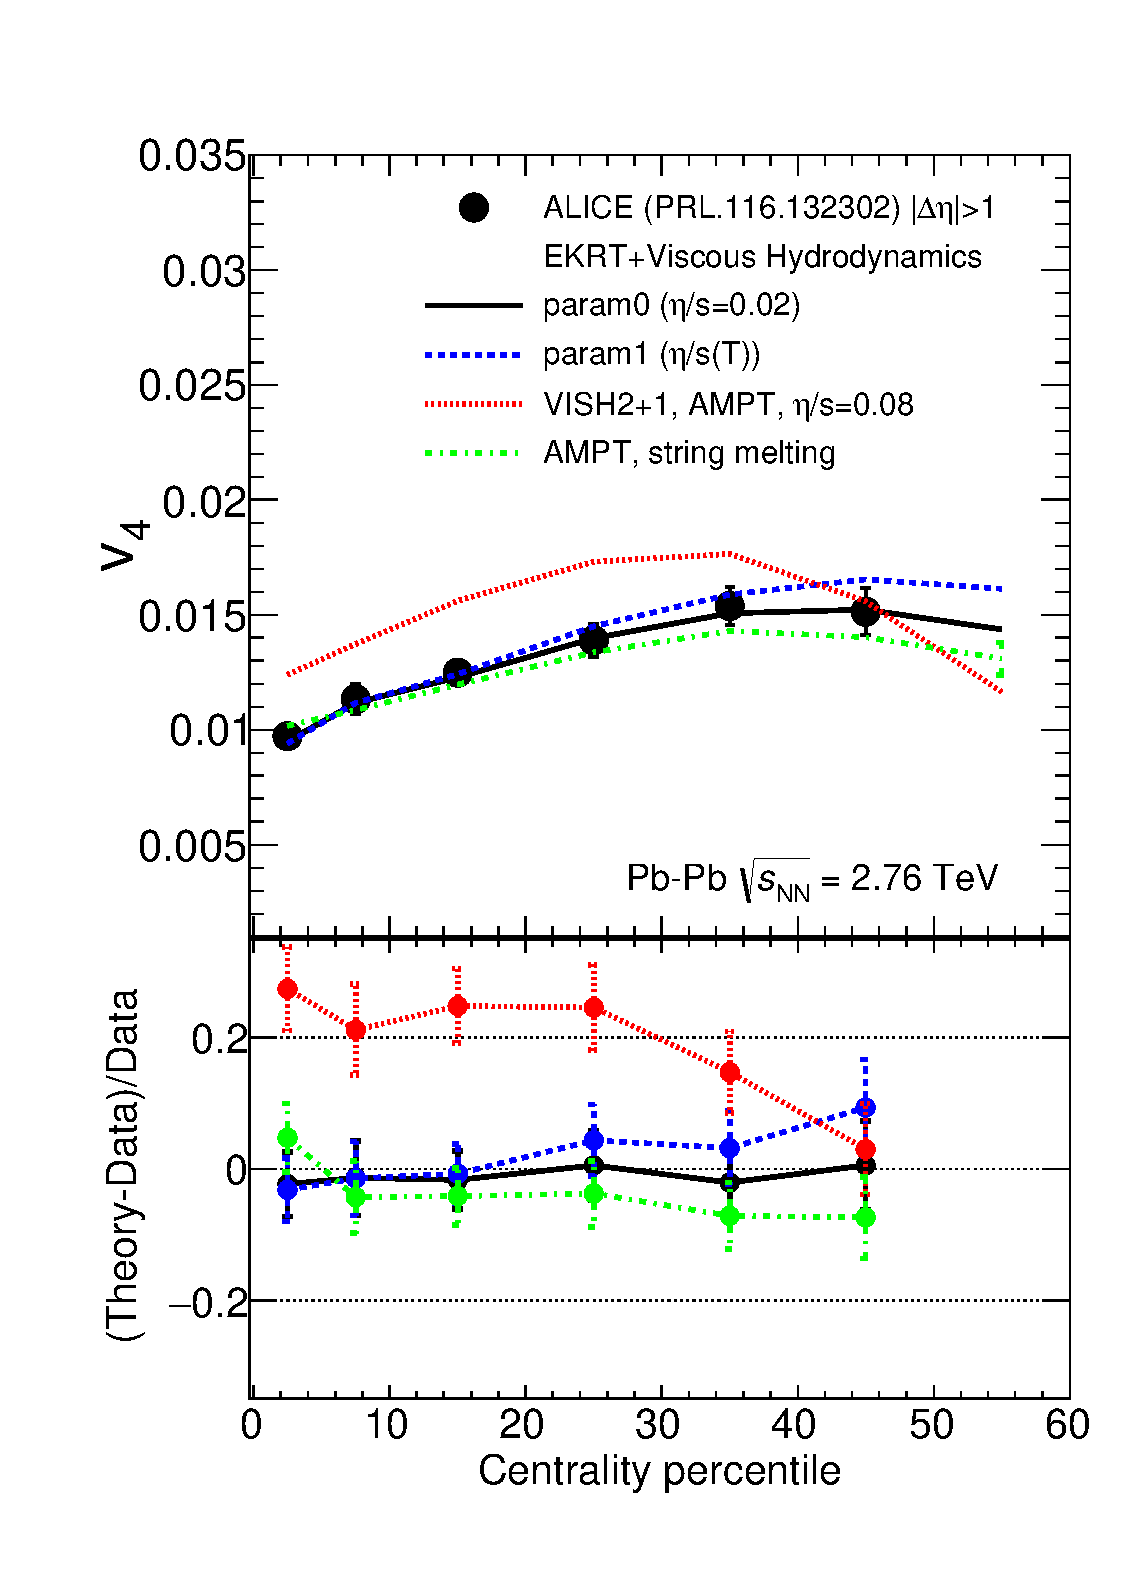
\includegraphics{figs/FigA4_v4_modelcomparisonBest.eps}}
        \caption{The individual flow harmonics $v_n$ (n=2, 3 and 4) in $\PbPb$ collisions at $\snn=2.76$~TeV~\cite{Adam:2016izf} are compared to few selected model calculations from three theoretical models which describe the $v_n$ data best.}
        \label{fig:Figure_A4}
              \end{center}
\end{figure*}

Finally, few selected calculations from three theoretical models which describe the $v_n$ data best are shown in Fig.~\ref{fig:Figure_A4}.
The calculations from the event-by-event EKRT+viscous hydrodynamic, VISH2+1 with AMPT initial conditions ($\eta/s$ =0.08) and the string melting version of AMPT give the best description of the individual flow harmonics $v_n$ (n=2, 3 and 4) with the accuracy of 5-20\% and the centrality dependence differs in three models as well as in different order flow harmonics.
The simultaneous description of all order individual flow harmonics $v_n$ is necessary to further optimize model parameters and put better constraints on the initial conditions and the transport properties of nuclear matter in ultra-relativistic heavy-ion collisions together with SC$(m,n)$ and NSC$(m,n)$.
